\documentclass[notoc,justified,openany]{tufte-book}    % `notoc` suppresses TL custom TOC, reverts to standard LaTeX
\usepackage{graphicx}
\usepackage{xspace}
\usepackage{hyperref}
\hyphenation{HMMER}
\newcommand{\hmmer}{{HMMER}\xspace}  % \hmmer is a command that expands to "HMMER" with a trailing space
\newcommand{\homot }{{Homot}\xspace}  % \homot  is a command that expands to "homot" with a trailing space
\newcommand{\Homot}{{Homot}\xspace}
\newcommand{\uniprot}{{UniProt}\xspace}
\newcommand{\userguide}{HMMER User's Guide}
\title{Homot: a Homology Observation Tool}
\subtitle{}
\author{Nicholas P. Carter, Sean R. Eddy}
\subauthor{}
\pkgurl{http://www.eddylab.org/software/homot/}
\pkgversion{1.0}   % ./configure replaces HMMER_VERSION
\pkgdate{November, 2026}         %    ... and HMMER_DATE

                    % definitions for \maketitle 
\bibliographystyle{unsrtnat-brief}   % customized natbib unsrtnat. Abbrev 3+ authors to ``et al.'' 

\begin{document}
\setcounter{tocdepth}{2}             % 0=chapters 1=sections 2=subsections 3=subsubsections? 4=paragraphs

\maketitle

\newpage
\begin{fullwidth}
  ~\vfill
  \thispagestyle{empty}
  \setlength{\parindent}{0pt}
  \setlength{\parskip}{\baselineskip}

\par
Copyright (C) 2026 Howard Hughes Medical Institute.

\par
HMMER and its documentation are freely distributed
under the 3-Clause BSD open source license. For a copy of the license,
see \href{https://opensource.org/licenses/BSD-3-Clause}{opensource.org/licenses/BSD-3-Clause}.

\par
HMMER development is supported in part by the National Human
Genome Research Institute of the US National Institutes of Health under
grant R01HG009116. The content is solely the responsibility
of the authors and does not necessarily represent the official views of
the National Institutes of Health.

\end{fullwidth}







\pagebreak
\hspace{0pt}
\vfill
\emph{\Homot is dedicated to the memory of Tom Jones: biologist, friend, and Player of Games. Tom was one of the inspirations for the development of \homot, but passed away before it was completed.  We hope that \homot will help others bring the curiosity, thoughtfulness, and joy to biology that Tom showed every day.}
\vfill
\hspace{0pt}

\chapter{Introduction}
\homot\sidenote{\homot was inspired by, and is heavily based on, the tools developed by the European Bioinformatics Institute for their web-based HMMER server \url{https://www.ebi.ac.uk/Tools/hmmer/home}. We are indebted to them for their work, and offer \homot as a complement to, not competition with, their tools.} is a graphical tool for the analysis and exploration of homology search results.  It displays search results in three ways: sorted by hit quality (e-value), distributed across a taxonomic tree, and grouped by structure (the set of domains or other annotated regions that a sequnece contains).  These views allow users to quickly grasp the breadth of the homologs a search has identified and zoom in on the results of greatest interest without having to pour through the thousands of results that searching a modern genomic database typically returns.

\homot takes two inputs: the output of a homology search run against a set of sequences that have been annotated for use with \homot, and an "annotations database" containing the annotations for that set of sequences.  \homot can display the results of HMMER (hmmsearch or phmmer), BLAST, or any other tool that can format its output to be compatible with HMMER's domtblout or BLAST's tabular output formats.  We provide annotations for a small set of genomic databases on Harvard's Dataverse at (FILL THIS IN).  \homot's source-code distribution also includes tools that users can use to annotate their own genomic databases, although this process can be somewhat complex.


\chapter{Installation}



\chapter{Usage}
When a user starts \homot, they are presented with the "select data" page show in Figure \ref{fig:load_data}\sidenote{Macintosh version shown. Linux and Windows versions may differ slightly.}.  This page contains a number of elements that are consistent across all of \homot's pages.  In the upper left of the window, the three-horizontal-line "hamburger"\sidenote{Flutter/Google's term, not ours} icon can be clicked to display a menu that allows users to see information about \homot, quit the application, or, once data has been loaded into the application, export displayed data to a {CSV} file.  Clicking the "gear" icon in the window's upper-right corner takes the user to \homot's settings page (described later), where the user can configure \homot's display and other application parameters.  At the bottom of the page, a navigation bar allows the user to switch between the \homot's different pages.  Icons in the navigation bar are greyed out when it is not possible to switch to the page, either because the user is already on that page, as is the case for the "Select Data" icon, or because no data has been into the application or selected for display, as is the case for the other icons in the figure.

\begin{figure*}
\centering
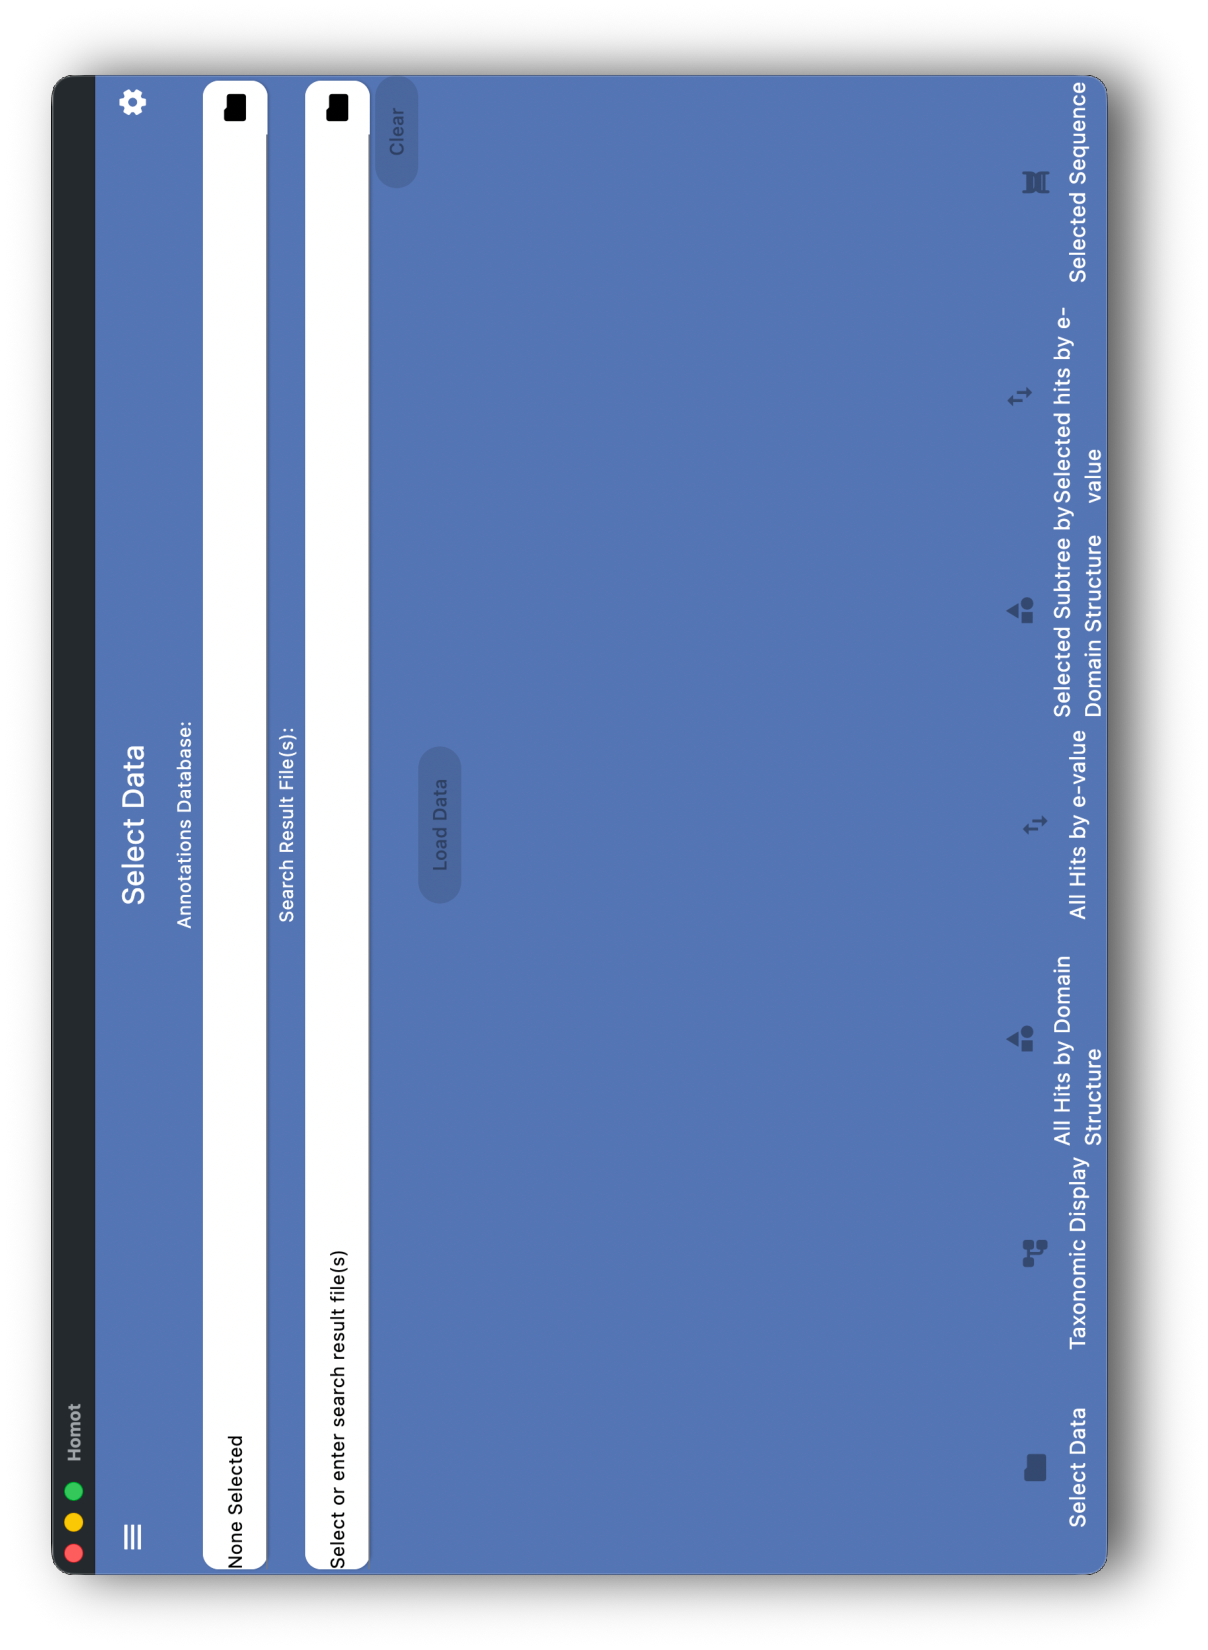
\includegraphics[width=\textwidth, angle=270]{inclusions/load_data.pdf}
\caption{\homot's Select Data Page}
\label{fig:load_data}
\end{figure*}

\homot requires two inputs in order to display search results: a file containing the results to be displayed, and an annotations database containing taxonomic and structure information about the database the search was run on.  To specify the annotations database that \homot should use, either type the location of the database into the corresponding text field or click the file folder icon at its right to bring up a file selector dialog and select the database.  Similarly, either type the location of the search results file you want to display in the "Search Results File(s)" field or click the file folder icon to bring up a file selector dialog that will allow you to locate the results file in your file system.

\homot accepts search results in either HMMER's domtblout format or BLAST's tabular (output format 6) format, and should be able to display results from other tools that can generate output in one of those formats.  Users may view the results of a single search, or of multiple searches against the same database to compare them.  By default, \homot infers the type of results file from its contents, but a Because HMMER and BLAST provide different information in their outputs, there will be some variation in the information displayed depending on the type of input file used.  All of the examples in this userguide show results from HMMER searches.

One note about annotation databases: an annotation database is a directory structure, not a flat file\sidenote{This is a result of our decision to use Rust's Fjall \url{https://docs.rs/fjall/latest/fjall/} key-value store to implement annotations databases.}.  When specifying the annotations database \homot should use, users should select the top-level directory of the database, not any of its sub-directories.

Once the user has specified an annotations database and one or more results files to display, they should click on the "Load Data" button to read the specified files into \homot.  Reading the input files takes between a few seconds for searches with a few thousand results to a few minutes for searches with millions of results, although this will vary with the speed of a computer's disk system.  While data is loading, \homot pops up a "Loading Data" message in yellow at the bottom of the screen.  If any problems occur loading the specified data, a red pop-up will appear containing an error message.  Otherwise, when the data finishes loading, \homot will switch to the taxonomic display page and show the search results.

\section{Taxonomic Display}
Figure \ref{fig:taxonomy} shows \homot's taxonomic display of search results.  Results are displayed on a circular graph, with the root at the center and successive levels of the taxonomy at increasing distances from the center.  Each node of the taxonomic tree occupies a fraction of the circle proportional to the fraction of the search's results that lie on that branch of the tree, and is colored based on which child of the root node it descends from, although other display formats can be selected from the settings page.  In the figure, for example, the bacteria occupy the majority the circle, as they contain 957 of the 1164 homologs found by the search, and all bacterial results are colored pink.  When there is sufficient space in the display, \homot represents a graph node as a radial line outward from its parent node, labeled with the name of the node and the number of results that are children of the node or the node's children.  When that is not possible \homot represents the node as a radial wedge extending out to the edge of the graph and labeled with the node's name and number of result, as it did for the Thermoproteati node in the figure, or as a colored radial wedge if the name and number of results do not fit.  One consequence of this is that \homot's initial display of search results often looks like a simple pie graph, as it shows all of the levels of the taxonomic tree by default, and most monitors do not have enough resolution to display node names when showing that many nodes.  Using the control in the upper-left of the window to reduce the number of graph levels displayed, as was done for the graph in the figure, will typically allow names to be displayed and more detail to be shown.

\begin{figure*}
  \centering
  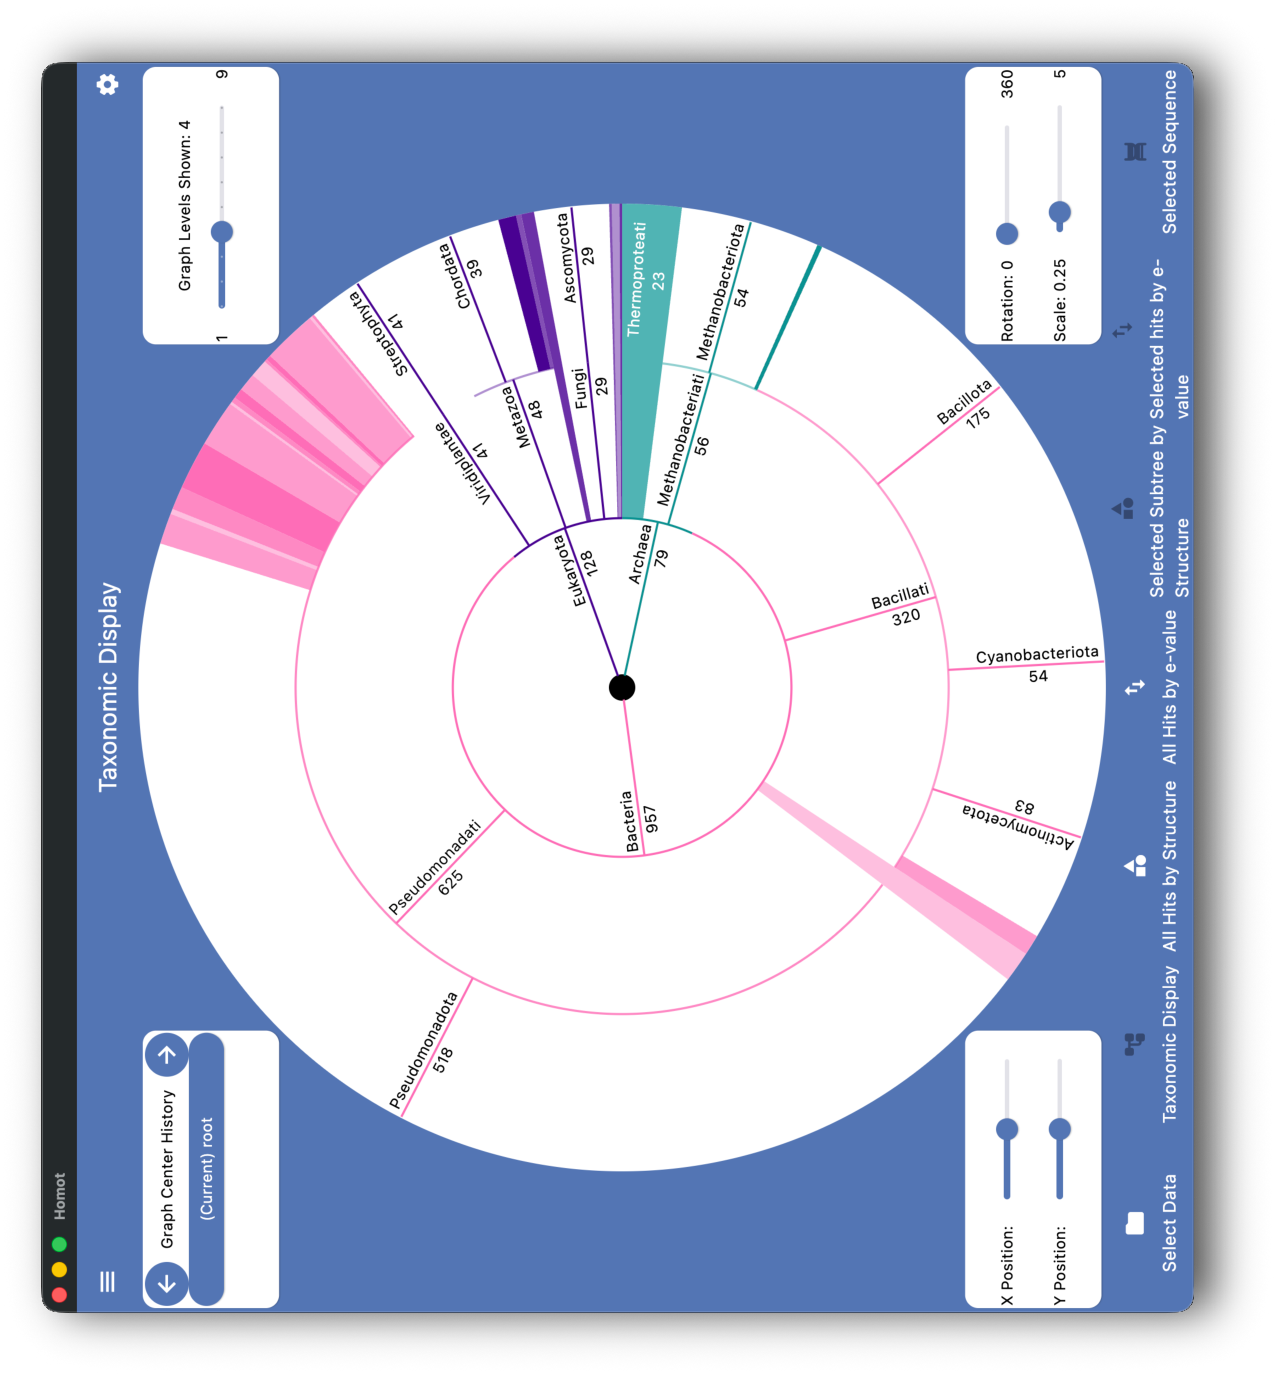
\includegraphics[width=\textwidth, angle=270]{inclusions/taxonomy.pdf}
  \caption{Taxonomic Display of Search Results}
  \label{fig:taxonomy}
  \end{figure*}

Left-clicking on a node in the graph makes that node the new root of the graph, allowing the user to show more detail about portions of the taxonomy that contain interesting results.  This also selects the results that are descendants of that node to be displayed on the "Selected Subtree by Structure" and "Selected hits by e-value" pages.  The control at the upper left of the window shows a history of the nodes that have been the center of the graph, and the user can return to a previously-selected center by clicking on its name in the control.  Right-clicking on a node brings up a pop-up that shows information about the node and allows the user to remove the node from the graph or view/restore nodes that have been removed from the graph.  Removing nodes from the graph can be useful when a node that contains a few results of interest takes up such a small fraction of the graph circle that it is hard to select.  In that case, removing one or more of the nodes that contain many results from the graph can expand the node of interest to the point where it can be easily selected.  Left-clicking anywhere outside the pop-up will close it, as will clicking the "close" button in the window.



\section{Grouping results by Structure}

\begin{figure*}
  \centering
  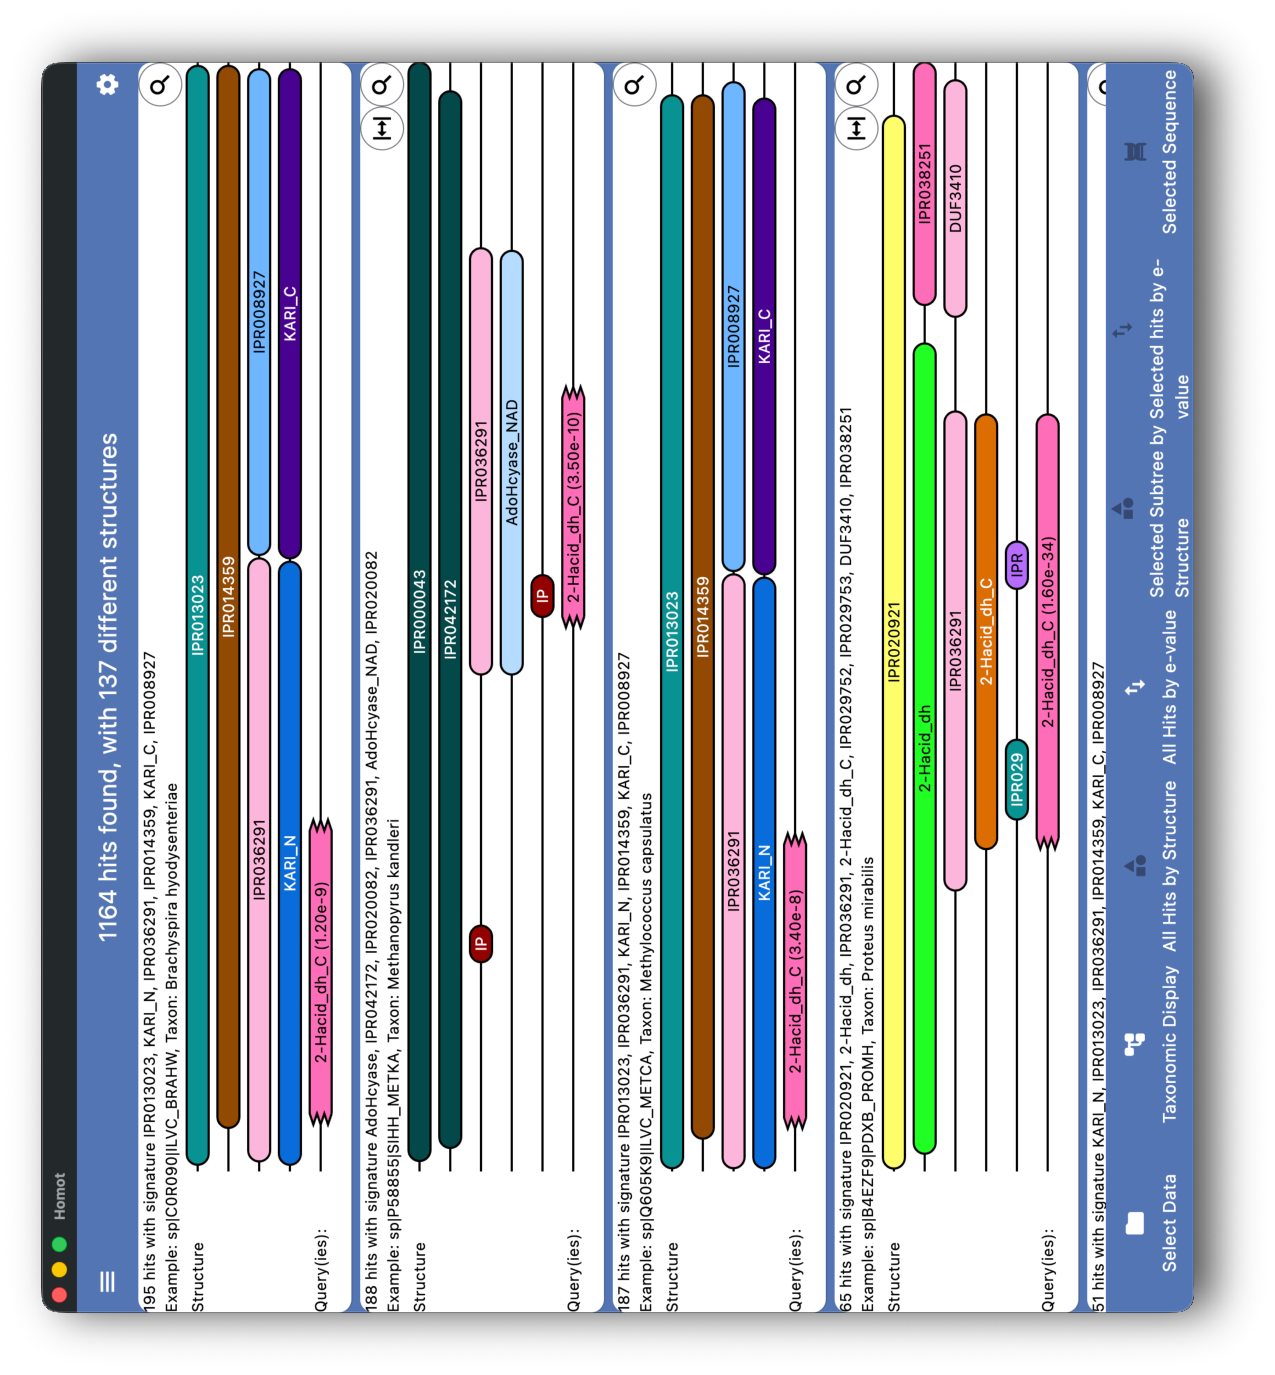
\includegraphics[width=\textwidth, angle=270]{inclusions/structure.pdf}
  \caption{\homot}
  \label{fig:structure}
  \end{figure*}

\section{Display by E-Value}
\begin{figure*}
  \centering
  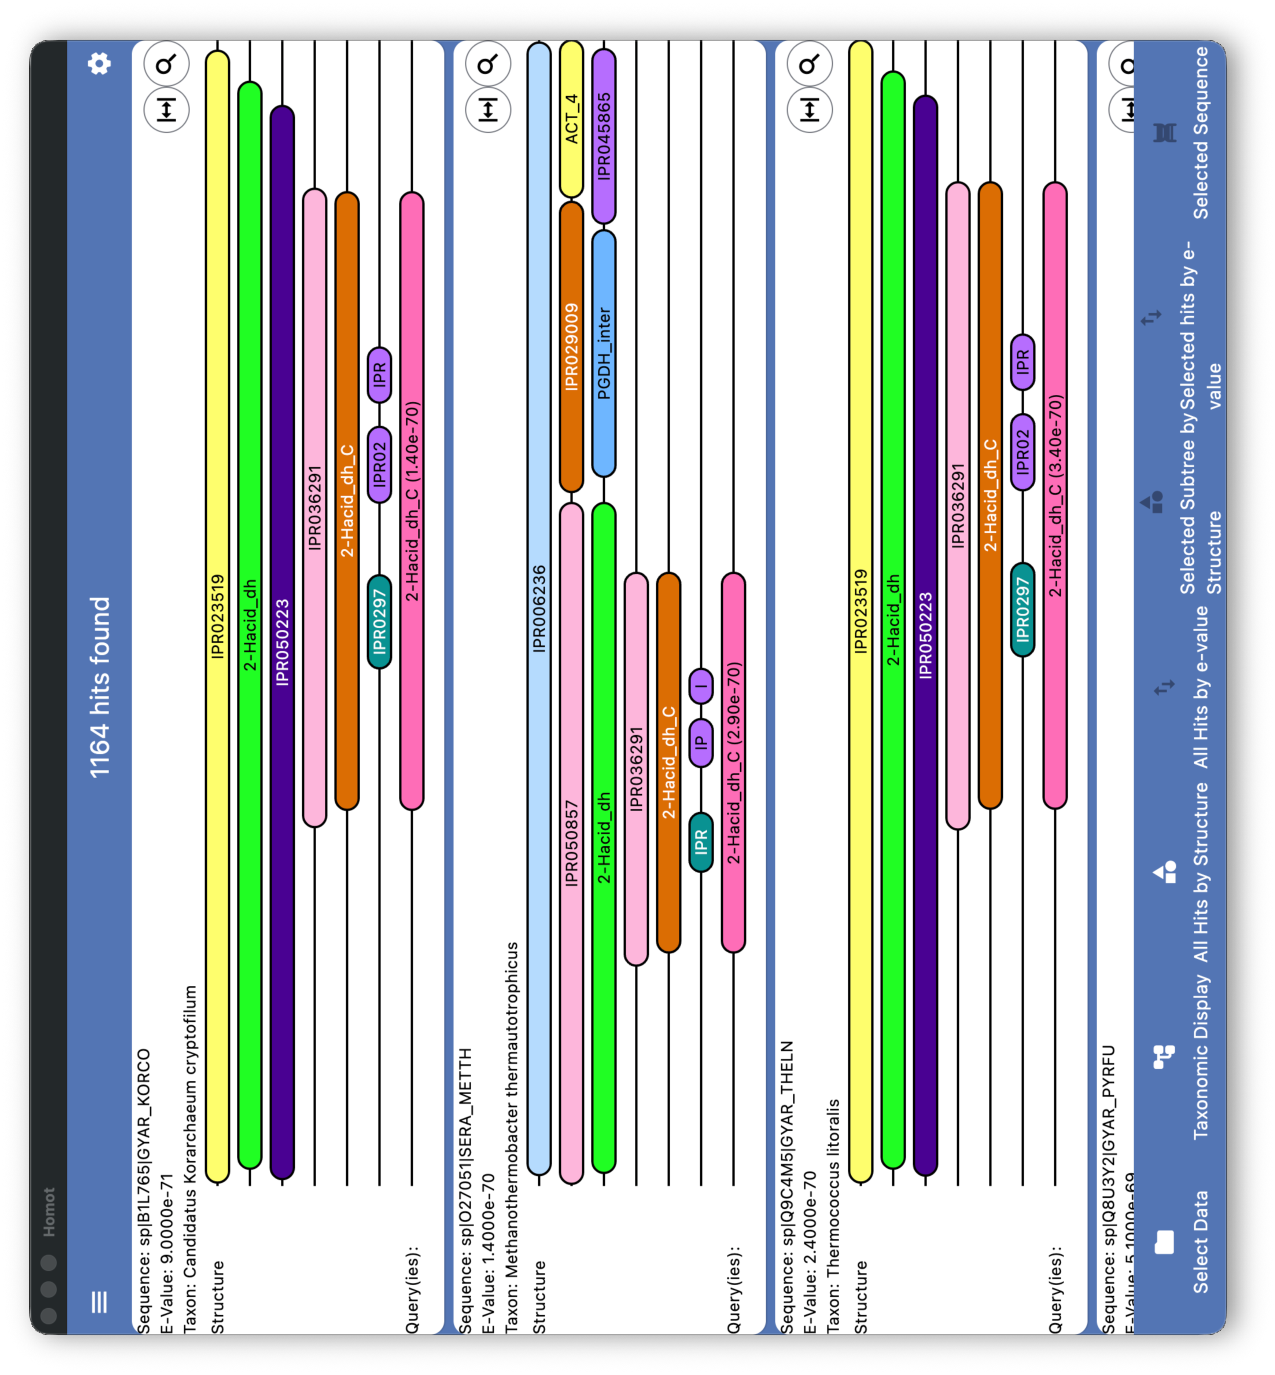
\includegraphics[width=\textwidth, angle=270]{inclusions/evalue.pdf}
  \caption{Sorting Resuts by E-Value}
  \label{fig:evalue}
  \end{figure*}

\section{Showing Individual Sequence Results}
\begin{figure*}
  \centering
  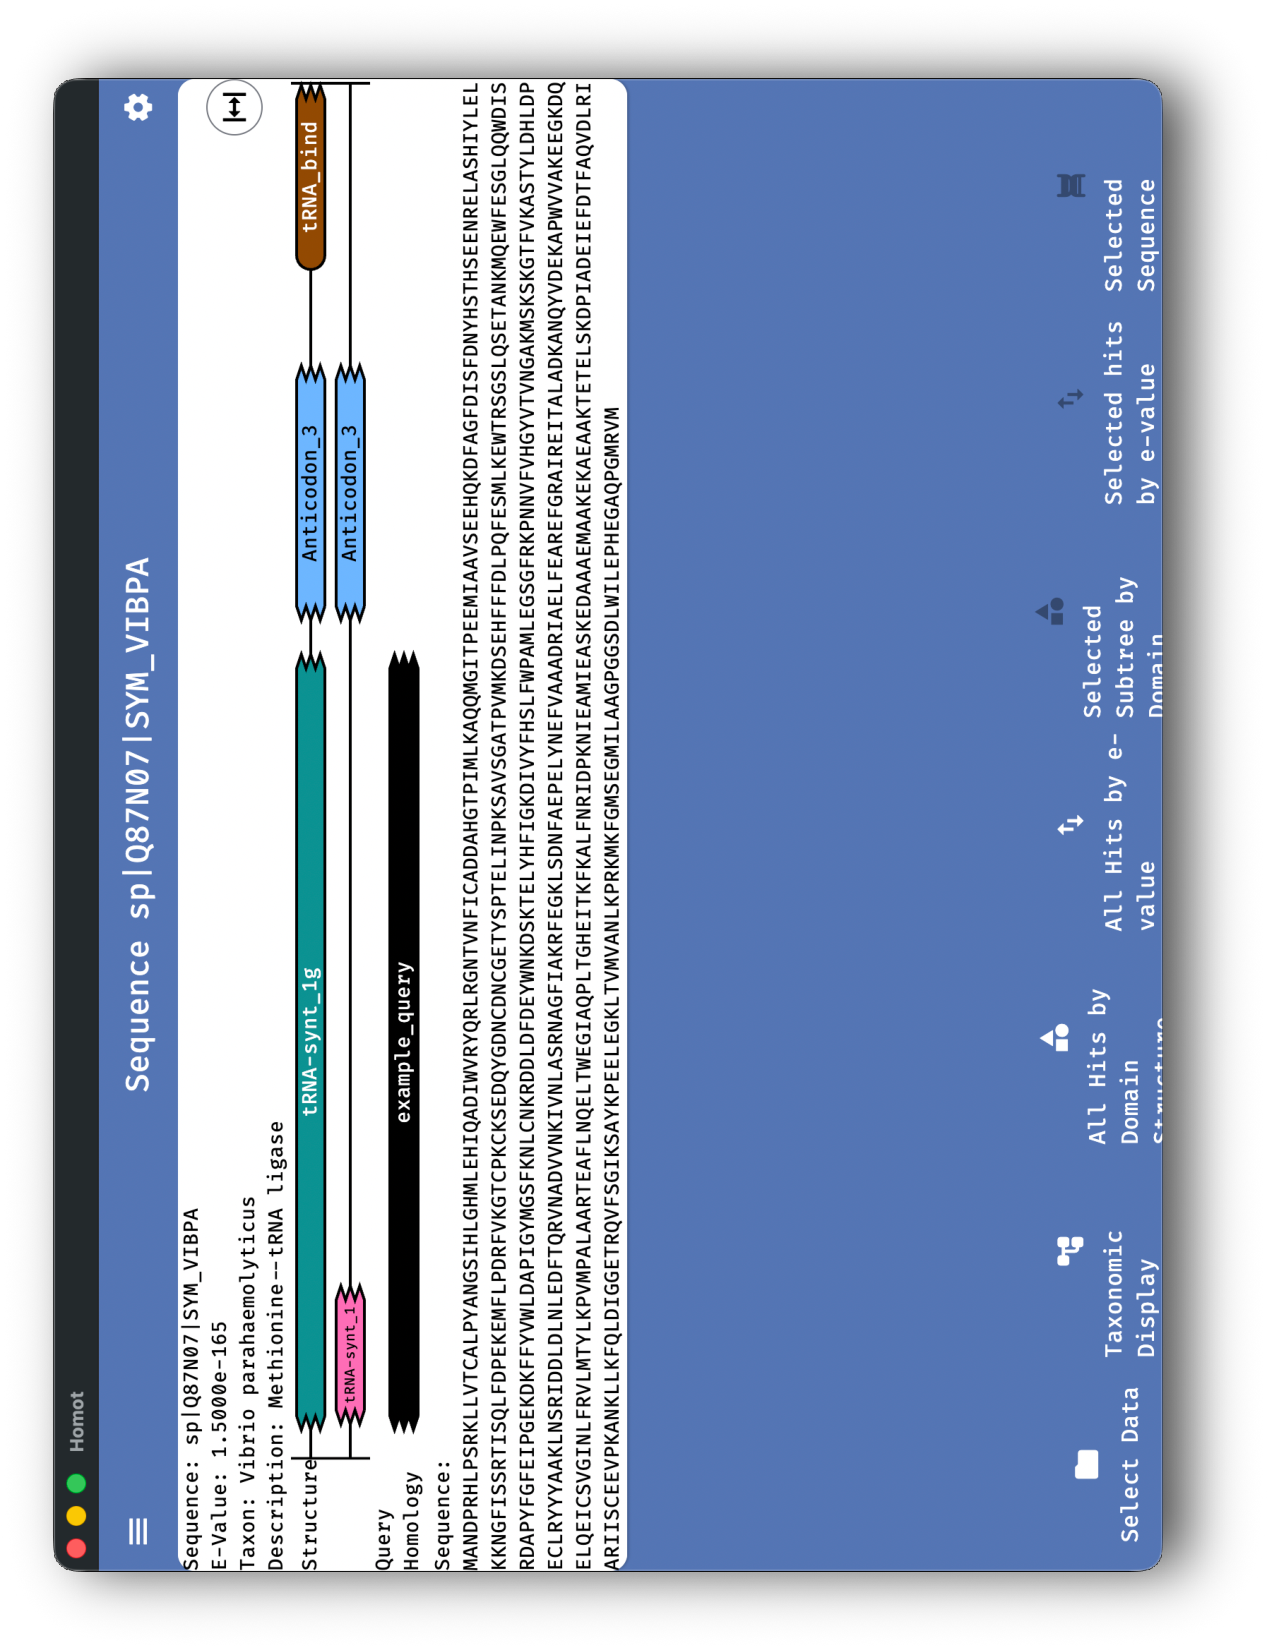
\includegraphics[width=\textwidth, angle=270]{inclusions/sequence.pdf}
  \caption{Single-Sequence Results}
  \label{fig:sequence}
  \end{figure*}

\section{Settings Screen}
\begin{figure*}
  \centering
  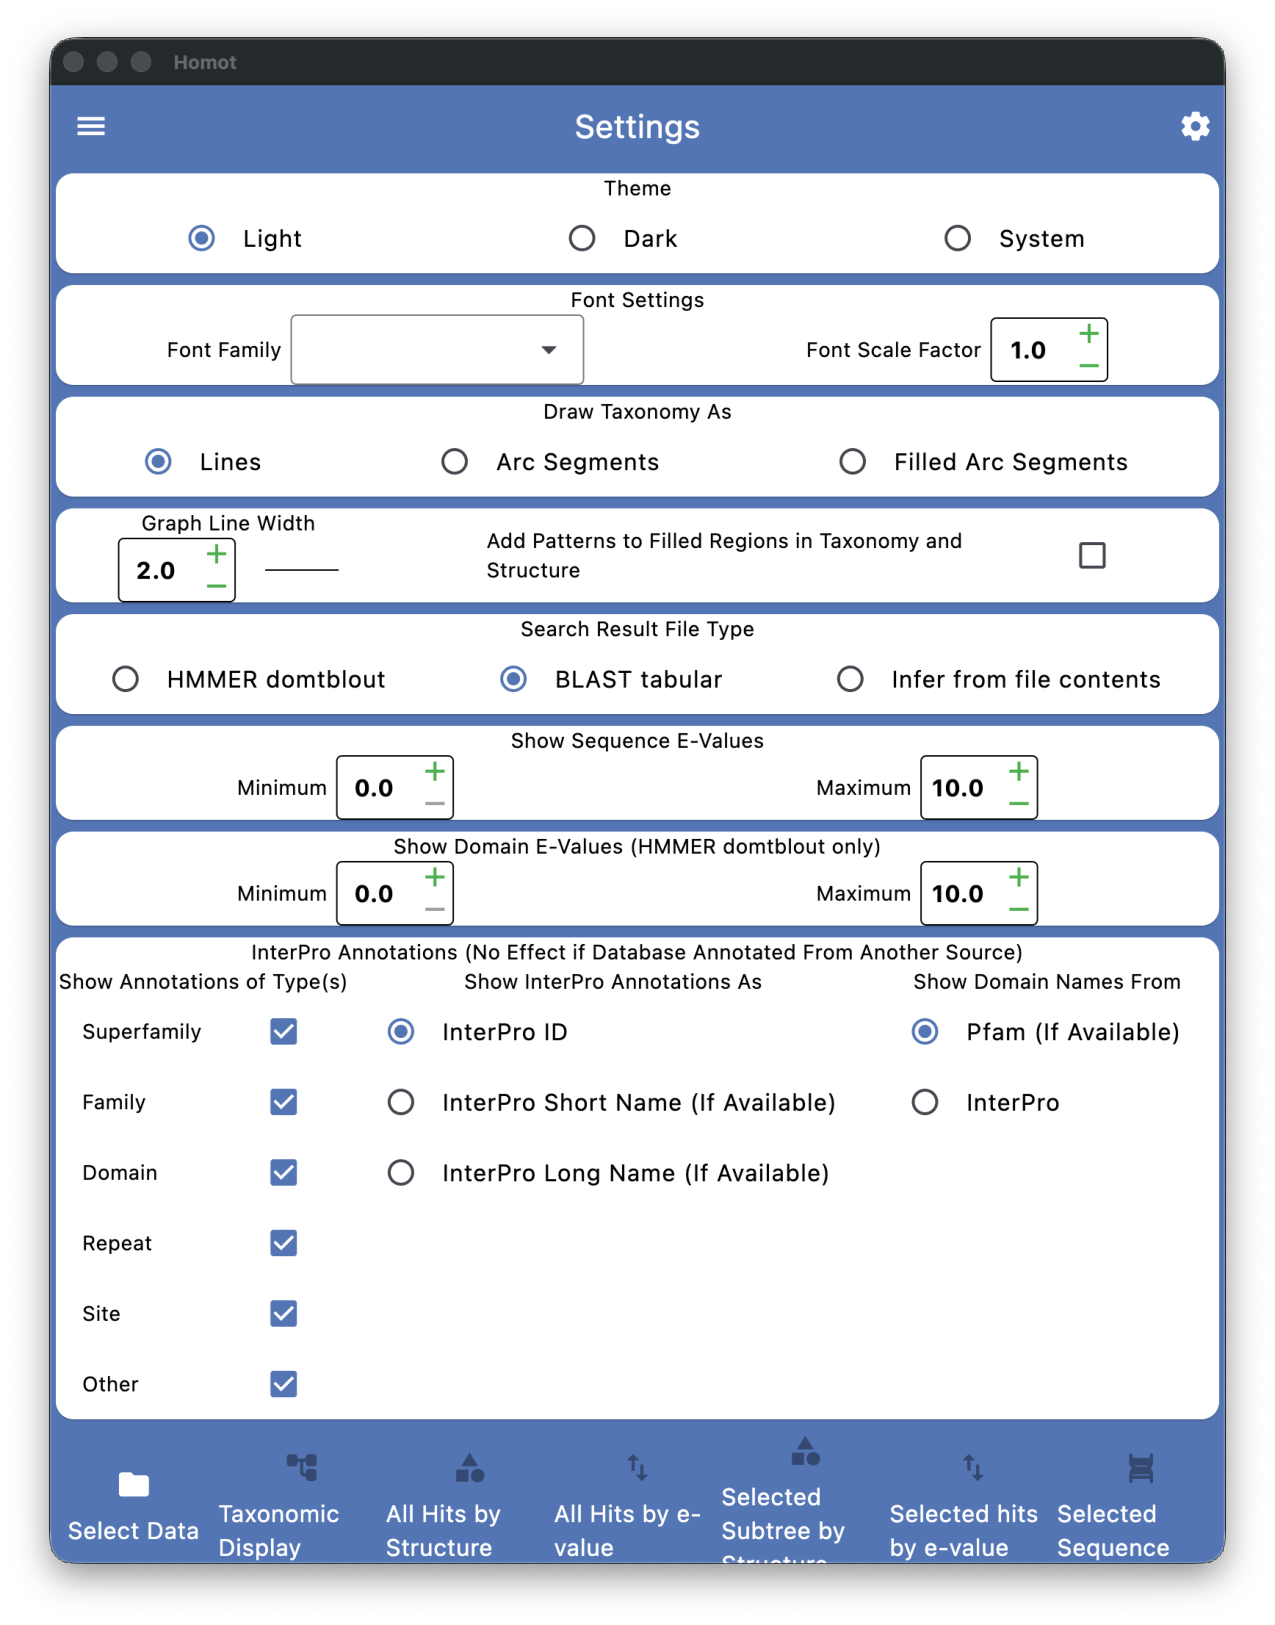
\includegraphics[width=\textwidth, angle=270]{inclusions/settings.pdf}
  \caption{\homot's Settings Page}
  \label{fig:settings}
  \end{figure*}

\chapter{Annotating Sequence Databases}
We provide two utilities to create annotations for files of protein sequence data.  The first, \mono{create\_annotations\_interpro}, annotates \uniprot \url{https://www.uniprot.org/} using the annotations that Interpro \url{https://www.ebi.ac.uk/interpro/} generates for those databases.  It is straightforward and fairly simple to run, but is limited to databases that Interpro annotates.  The second, \mono{create\_annotations\_hmmer}, annotates arbitrary databases against the domains defined by Pfam \url{http://pfam.xfam.org/} or other sets of HMMs, but requires significantly more preparation to use.  Both are included in the source-code distribution of \homot, which is available at (SITE GOES HERE).  

Building these tools from source is fairly simple.  Both are written in the Rust language \url{www.rustup.rs}, and require that to be installed.  Once Rust has been installed on your system, clone the \homot Git repository, change into the \mono{create-annotations} directory inside of it, and run "cargo build --release".  Cargo should download all of the required dependencies for you, build the two tools, and deposit them in the \mono{create-annotations/target/release} directory of the repository.  


\section{Data Required to Create Annotations}
Creating an annotations database requires a number of input files.  The first is the FASTA database to be annotated.  Our annotation tools expect each sequence in the database to specify its NCBI taxon ID using the "OX=taxid" format defined by \uniprot.  \uniprot databases will contain that information, but databases from other sources may have to be modified to add it.  If this information is not available, an annotations database can still be created, and the structure display functions of \homot will still work, but the taxonomic display will not (all sequnces will be placed at the taxonomy's root node).  Another note about taxonomic IDs is that the NCBI taxonomy changes very quickly and \uniprot does not say which version of the taxonomy was used when creating a given version of their databases, so there will generally be a small number (hundreds out of many millions) of sequences in a \uniprot database whose taxon IDs no longer exist.  \homot handles this by placing any such sequences at the root of the taxonomic tree.

By default, our annotation tools compress the NCBI's hierarchy (34 levels at the time of this writing) into the canonical hierarchy of domain, kingdom, phylum, class, order, family, genus, species, with "no rank" for nodes at the very root of the hierarchy.  Passing the \mono{-n} option to the annotation tool will prevent this, leaving the hierarchy at its full depth.

Both annotation tools use the NCBI taxonomy \url{https://www.ncbi.nlm.nih.gov/taxonomy} to place results on the tree of life.  To do this, they expect the taxonomy definition files \mono{names.dmp}, \mono{nodes.dmp}, \mono{merged.dmp}, and \mono{delnodes.dmp} to be located in the same directory.  These files can be obtained by downloading the file \mono{taxdump.tar.Z} from the NCBI's FTP site at \url{https://ftp.ncbi.nlm.nih.gov/pub/taxonomy/}, and un-compressing and un-tarring that file.

Annotating a \uniprot database with Interpro annotations requires the \mono{interpro.xml} and \mono{protein2ipr.dat} files for the appropriate release of Interpro, which can be downloaded from \url{https://ftp.ebi.ac.uk/pub/databases/interpro/}, and should be placed in the same directory.  Each Interpro annotation release corresponds to a \uniprot release, so it should be possible to locate the Interpro annotations that match any given database.

Annotating a sequence database with Pfam domains requires the \mono{{Pfam-A.clans.tsv}} and \mono{{Pfam-A.hmm}} files for the appropriate Pfam release, which can be downloaded from \url{https://ftp.ebi.ac.uk/pub/databases/Pfam/current_release/}.  Again, both files should be placed in the same directory.  

\section{Annotating \uniprot Databases with Interpro Annotations}
Once all of the required data files have been assembled, a \uniprot database can be annotated with the Interpro annotations using the command "create\_annotations\_interpro <seqfile> <interprodir> <ncbidir> <outfile>", where <seqfile> is the FASTA file to be annotated, <interprodir> is the directory containing the Interpro datafiles, <ncbidir> is the directory containing the NCBI taxonomy information, and <outfile> is the desired name for the annotations database.  Annotating a FASTA file contaning 200 million sequences this way takes less than an hour on a 2025 Mac Studio computer.

\section{Annotating Databases with Pfam Domains}
Annotating a sequence database with Pfam domains is more complex, but more flexible.  In addition to the input files described above \mono{create\_annotations\_hmmer} requries a directory of \hmmer domtblout files, one per domain that Pfam defines, which contain the hits to that domain from the sequences in the database.  The easiest way to generate these files is to separate the {Pfam-A.hmm} files into individual {HMM} files, one per domain, and then to run a HMMER search on each of those files using commands similar to "hmmsearch --cut\_ga --domtblout=domtbldir/domain.domtblout sequences.fasta", where the --cut\_ga option instructs hmmsearch to use the Pfam reporting thresholds contained in the {HMM} file.  One requirement here is that the domtblout files be named with the name of the domain they represent, as \mono{create\_annotations\_hmmer} uses that when creating the annotations.

Once that has been done, which can take a significant amount of time depending on the number of machines available to run all of the HMMER searches, the database can be annotated using the command "create\_annotations\_hmmer <seqfile> <domtbloutdir> <pfamdir> <ncbidir> <outfile>", where seqfile is the FASTA file to be annotated, domtbloutdir is the directory containing the above domtblout files, pfamdir is the directory containing the pfam data files, ncbidir is the directory containing the ncbi datafiles, and outdir is the name of the annotations database.  This can take a significant amount of time and RAM to run, depending on the size of the FASTA file being annotated.

This process can be adapted to annotate a database with hits to an arbitrary set of {HMM}s by generating domtblout files by searching the database against each HMM as above, collecting the {HMM} files into one "{Pfam-A.hmm}" file and creating a \mono{{Pfam-A.clans.tsv}} that is empty or contains relationship specifications for the {HMM}s being searched. \mono{Create\_annotations\_hmmer} expects that many Pfam domains will not be members of clans, so any {HMM}s not contained in the \mono{{Pfam-A.clans.tsv}} file will simply be treated as clanless.  Once this has been done, the database can be annotated using the same command as for a Pfam annotation.
\end{document}